\addchap{\enquote{Vorwort} oder \enquote{Was ist das hier?}}


Hallo! Bis hierher hast du es nun schon mal geschafft. Wohnungssuche und Umzug sind eben -- oder noch nicht mal -- vorbei, da hat das drohende Studium jetzt wahrscheinlich gerade noch gefehlt.

Doch was ist dieses \enquote{Studieren} überhaupt? Und wie geht das eigentlich? Mit der Erstsemestereinführung (ESE) wollen wir in der kommenden Woche ein wenig Licht ins Dunkel bringen.

%Du wirst schnell merken, dass das studentische Leben nicht mit dem Verlassen des Hörsaals endet. Ganz im Gegenteil: Wenn du dem grauen Alltag ein wenig entrinnen möchtest, wirst du in den 13 Dresdner Studentenclubs -- wie unter anderem dem Count Down in der Johannstadt -- und bei zahlreichen Ersti-Partys Gelegenheit finden.

%Du willst in einer Freistunde einfach nur ein wenig Koffein tanken? Na dann schau doch mal auf eine kolle-Mate -- den Dresdner Konkurrenten der Club Mate -- im \texttt{ascii} vorbei, dem Studentencafé der Fakultät.

Bei Spiel, Spaß und Spannung wirst du deshalb in den kommenden Tagen einiges an Information abbekommen. Um in der Flut nicht ganz untergehen, wollen wir das Wichtigste in diesem kleinen Heftchen hier bündeln.

Wie melde ich mich für Prüfungen an?  Wie ist mein Studium aufgebaut? Warum ist die Banane krumm? Welche Stipendien gibt es?
Einige dieser Fragen und noch viele weitere versucht dieses bescheidene Heftlein zu beantworten. %Das Motto ist klar: \textbf{Keine Panik!} (oder wenigstens nur ein moderates Ausmaß)

\textbf{Bleibt nur noch zu sagen: Viel Spaß in der ESE und im Studium!}

\begin{figure}[b!]
	\centering
	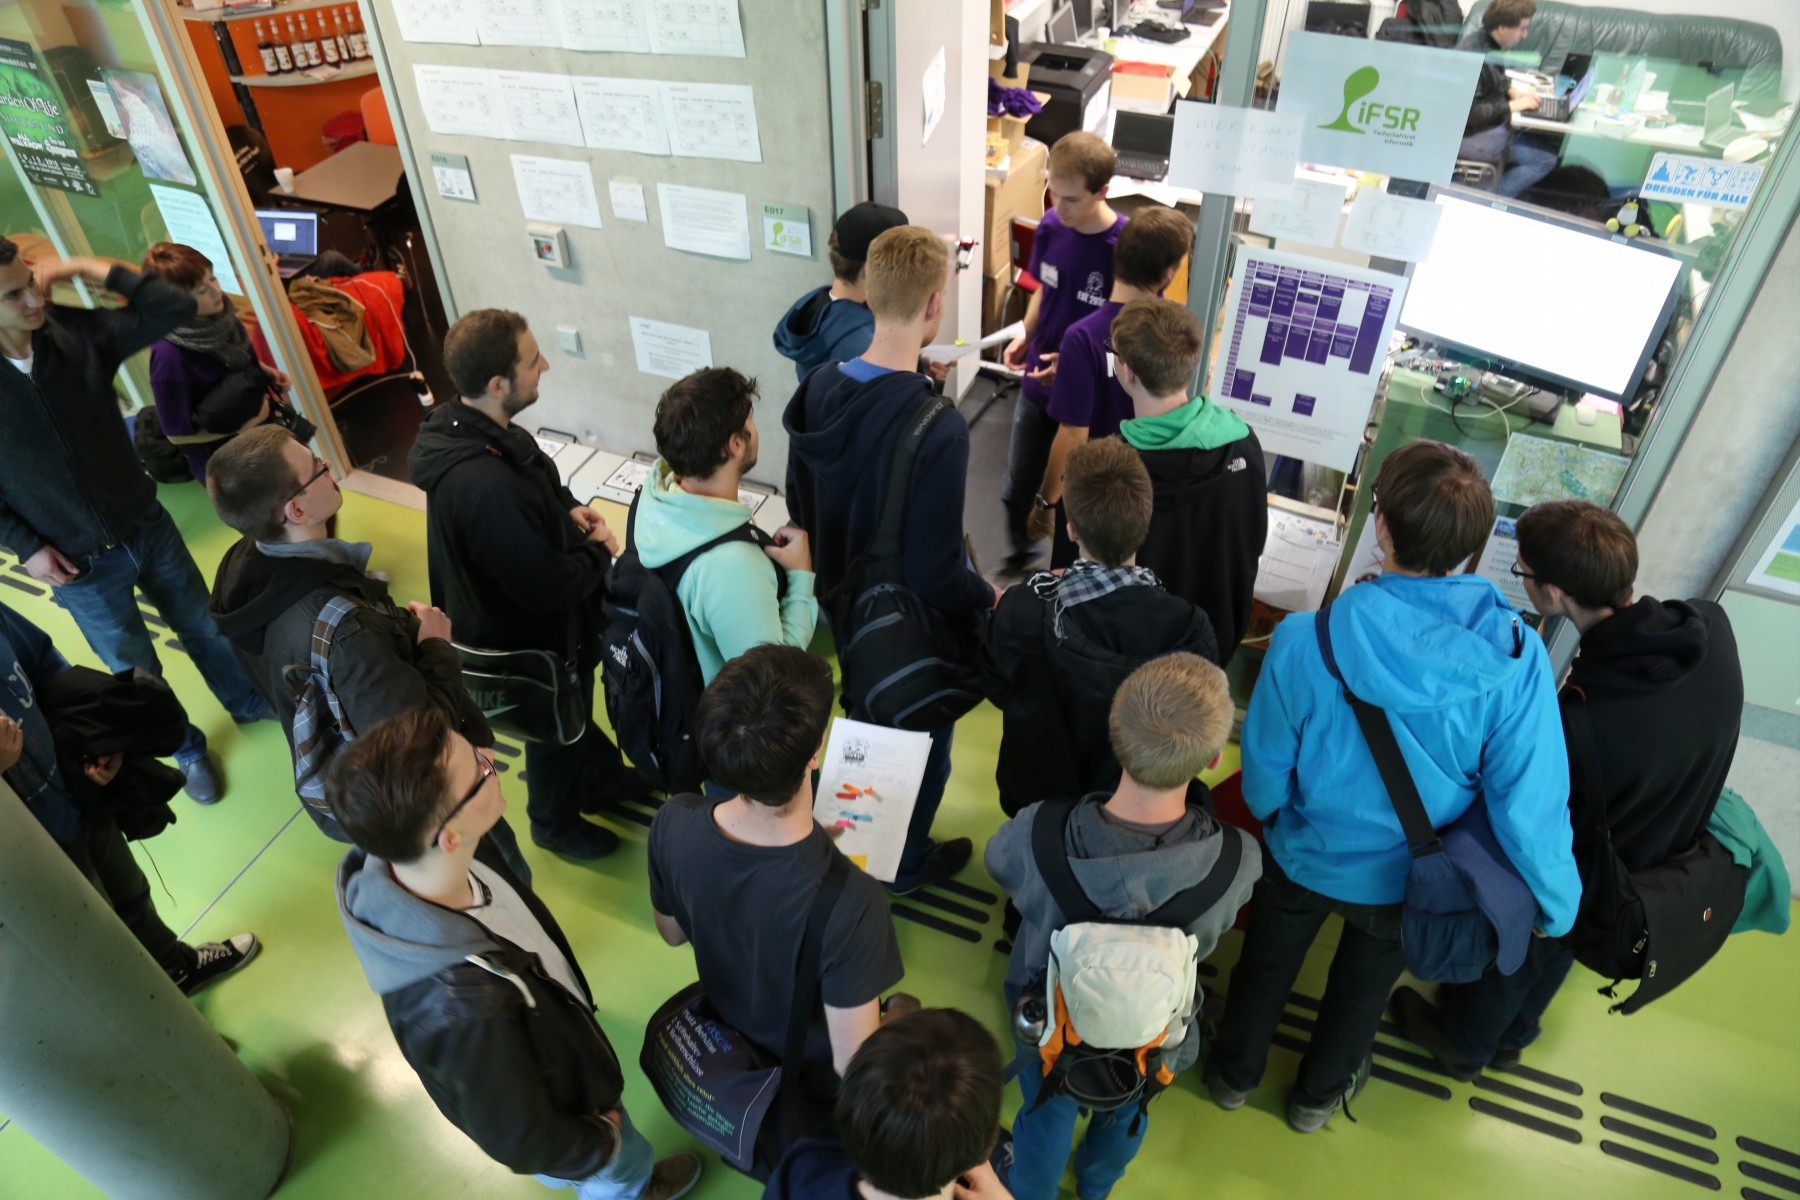
\includegraphics[trim={0 5.5cm 0 0}, clip, width=\linewidth]{img/ese2015/bueroansturm.jpg}
\end{figure}%

\bigskip
{\small PS\@: Links schauen in diesem Heft so aus: \link{https://html5zombo.com}. Ganz hinten auf einer der letzten Seiten annst du dann die Adresse nachsehen. Ebenfalls kannst du auch direkt unter \url{ese.ifsr.de/2019/<Zahl>} auf die verlinkte Seite weitergeleitet werden.}
